% Multi-dimensional examples
\subsection{Higher Dimensions}
Having looked at one dimension, how well do these algorithms 
generalize to higher dimensions?

%%%%%%%%%%%%%%%%%%%%%%%%%%%%%%%%%%%%%%%%%%%%%%%%%%%%%%%%%%%%%%%%%%%%%%%
% The distance to a point test cases.
\subsubsection{Dimensionality}
Considering that many problems, such as parameter estimation, actually
involve arms from some dimension higher than $\mathbb{R}$, it is
worth seeing how these algorithms generalize to higher dimensions.

Our first example of a bandit problem where the arms are
multi-dimensional is that of trying to find a point in the unit hypercube.
More specifically, we consider the $n$-dimensional hypercube, fix some
point $\mathbf{p}$ in it, and the reward function is defined as
\[
	r_p(\mathbf{x}) = \frac{1}{1 + dist(\mathbf{p}, \mathbf{x})}
\]
Note that this reward function has value 1 when $\mathbf{x} =
\mathbf{p}$, and gets arbitrarily close to 0.  It is also quite
smooth.  We plot the $\mathcal{X}$-armed algorithm against the
discretized $\epsilon$-greedy algorithm in \figref{fig:smoothness}.

\begin{figure}[!ht]
  \begin{center}
    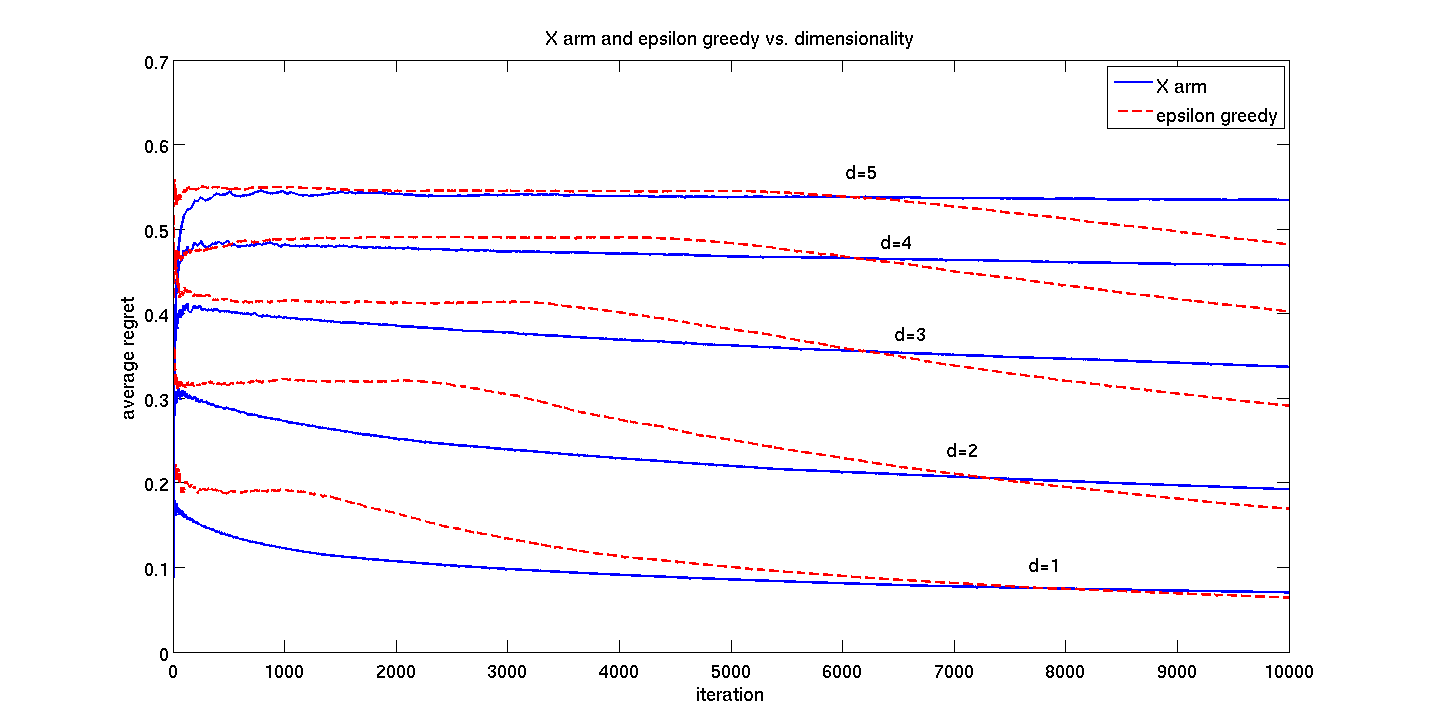
\includegraphics[width=\figwidth]{figures/dimensionComparison}
     \caption{Comparison of HOO and $\epsilon$-greedy algorithms
       distance payoff function for various dimensionalities. The
       discretization uses $100 \cdot d$ arms.}
     \label{fig:smoothness}
  \end{center}
\end{figure}

Most obvious is the fact that both algorithms do worse in the same
number of trials when the dimension is increased.  For the
$\epsilon$-greedy algorithm, this occurs because its discretization
essentially gets coarser and coarser as the number of dimensions
increases.  However, the convergence of any of these discretization
algorithms is independent of the number of dimensions.  Similarly, the
$\mathcal{X}$-armed algorithm does worse with higher dimension simply
because the space is bigger and therefore it takes longer to explore.
However, unlike the discretization algorithms, the $\mathcal{X}$-armed
algorithm should converge to a zero average regret arm given enough
time.  The downside is that the computational complexity of the
$\mathcal{X}$-armed algorithm makes it infeasible to actual run enough
rounds to converge.  Practically, running that many rounds also
becomes an issue for any real-life scenario.

%%%%%%%%%%%%%%%%%%%%%%%%%%%%%%%%%%%%%%%%%%%%%%%%%%%%%%%%%%%%%%%%%%%%%%%
% Tic-Tac-Toe
\subsubsection{Learning a Tic-Tac-Toe AI}
To consider a slightly less abstract example of a reward function,
consider the problem of trying to design an AI for Tic-Tac-Toe.  In
particular, this AI takes the form of assigning a weight to each of
the nine squares on the board, and whenever it is the AI's turn in a
game it places its X or O in the square on the board with the highest
weight of the open squares.  The reward for a particular arm is
determined by playing against a random player, with reward 1 if the AI
wins, .5 if the game results in a tie, and 0 if the AI loses.  The
player who makes the first move in the game is decided at random.
Note that this reward function is piecewise constant, with noise, and
that the arms live in $\mathbb{R}^9$, a high-dimensional space.  As it
is somewhat unclear how well the best possible Tic-Tac-Toe AI would
do, we define `regret' in this scenario as simply $1-\text{reward}$,
even though average regret obviously can never approach zero.  As a
reference point, one AI that never loses (although it does not
necessarily maximize reward), achieves regret of about .14 under this
metric.  Now we examine how the algorithms did.

\begin{figure}[!ht]
  \begin{center}
    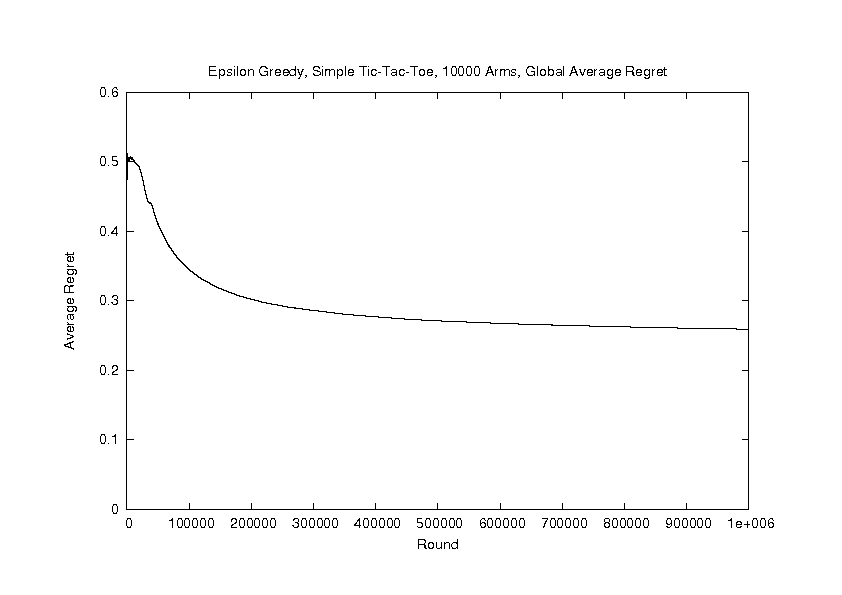
\includegraphics[width=\figwidth]{data/tictactoe/egtoe10000_GA.png}
     \caption{$\epsilon$-greedy algorithm on the Tic-Tac-Toe bandit with
     10000 arms}
     \label{fig:egtoe}
  \end{center}
\end{figure}

With 10000 arms, the $\epsilon$-greedy algorithm takes a while to
converge, compared to lower-dimension examples, but since the domain
the problem is over is so high, it's reasonable that we would want a
large number of arms in order to get something good.  Note that we can
run any of the discretization algorithms for a long time, since their
running time is $O(KT)$, with $K$ the number of arms and $T$ the
number of rounds.  The other discretization algorithms were also tried
out, but they did not behave significantly differently from the
$\epsilon$-greedy algorithm except in that parameters had to be chosen
for them so that they converged in a reasonable amount of time.  The
set of weights that the $\epsilon$-greedy algorithm converged to
on one trial is:
\[
\left(
\begin{array}{ccc}
0.937 & 0.490 & 0.673 \\
-0.969 & 0.125 & -0.248 \\
-0.741 & -0.367 & 0.007
\end{array}
\right)
\]
This makes sense, as the AI tries to make a 3-in-a-row right away,
which works frequently due to playing against a random player.  If the
game is still going on, then the AI tries to make 3-in-a-rows using
squares that it is already likely to have taken.

\begin{figure}[!ht]
  \begin{center}
    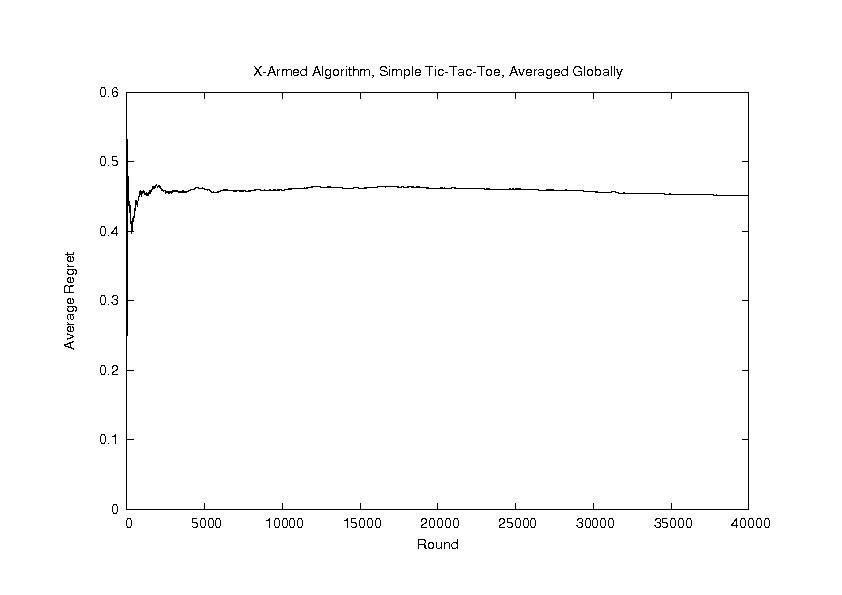
\includegraphics[width=\figwidth]{data/tictactoe/xarmtoe_GA.png}
     \caption{$\mathcal{X}$-armed algorithm on the Tic-Tac-Toe bandit}
     \label{fig:xarmtoe}
  \end{center}
\end{figure}
The $\mathcal{X}$-armed algorithm does not fare as well.  Due to the
high dimension of the arms, the algorithm remains exploring for a long
time and we run into computational issues before the algorithm starts
converging.

\begin{figure}[!ht]
  \begin{center}
    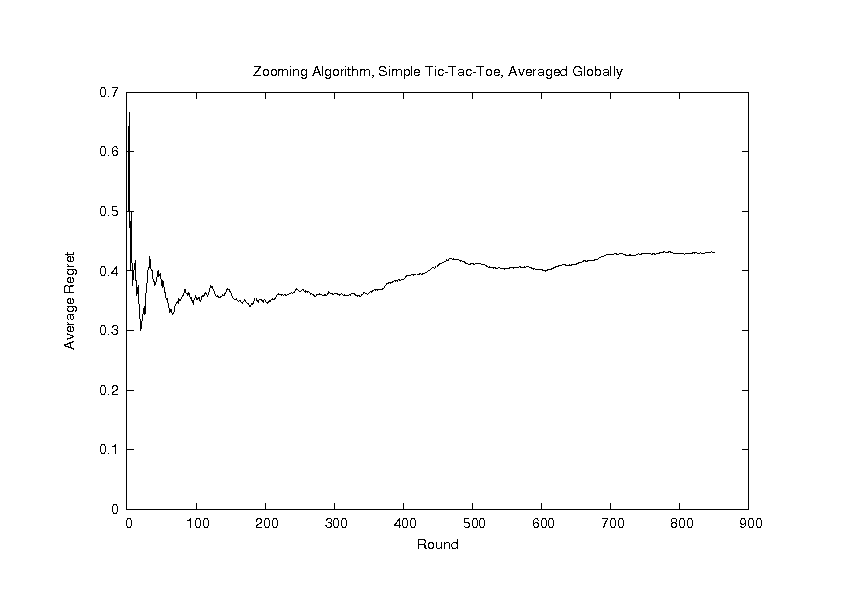
\includegraphics[width=\figwidth]{data/tictactoe/zoomtoe_GA.png}
     \caption{Zooming algorithm on the Tic-Tac-Toe bandit}
     \label{fig:zoomtoe}
  \end{center}
\end{figure}
The Zooming algorithm does worst of all.  This is due to the
horrendous complexity involved with a covering oracle in 9 dimensions,
which makes it completely impractical to run very many rounds at all.

From this example, we can see that, given a non-smooth problem in a
very high dimension, it may be better to simply use a discretization
algorithm, as the $\mathcal{X}$-armed algorithm will take too long to
converge and the Zooming algorithm will take too long to compute.
